\documentclass[aspectratio=169, table]{beamer}

%\usepackage[beamertheme=./praditatheme]{Pradita}
\usepackage[utf8]{inputenc}

\usetheme{Pradita}

\subtitle{MTI102-Information Systems \&\\Technology Architecture}

\title{Phase A:\\Architecture Vision in TOGAF\\Architecture Development Method}
\date[Serial]{\scriptsize {PRU/SPMI/FR-BM-18/0222}}
\author[Pradita]{\small {\textbf{Alfa Yohannis}}}

\begin{document}

    \frame{\titlepage}

    \begin{frame}
        \frametitle{Goals}
%        \framesubtitle{\hspace{1cm}}
        \begin{enumerate}
            \item Develop an aspirational (high-level) vision of the capabilities and business value that will be delivered as a result of the proposed enterprise architecture.
            \item Obtain approval for an Architectural Statement of Work that defines the work program to develop and implement the architecture outlined in the Architectural Vision.
        \end{enumerate}
    \end{frame}

    \begin{frame}
        \frametitle{Input}
%        \framesubtitle{\hspace{1cm}}
        \begin{enumerate}
            \item Request for Architectural Work
            \item Business principles, business goals, and business drivers
            \item Organizational Models for Enterprise Architecture
            \item Customized Architectural Framework, including architectural principles
            \item Populated Architecture Repository; i.e., existing architecture documentation (framework description, architecture description, existing baseline description, etc.)
        \end{enumerate}
    \end{frame}

    \begin{frame}
        \frametitle{Steps}
%        \framesubtitle{\hspace{1cm}}
        \begin{enumerate}

            \item \textbf{Creating an architectural project}
            \item \textbf{Identifying stakeholders, concerns and business requirements}
            \item Confirm and \textbf{develop} business goals, business drivers, and constraints
            \item Evaluate business capabilities
            \item Assess readiness for business transformation
            \item Defines the scope

        \end{enumerate}
    \end{frame}

    \begin{frame}
        \frametitle{Steps (2)}
%        \framesubtitle{\hspace{1cm}}
        \begin{enumerate}
            \setcounter{enumi}{6}
            \item Confirm and \textbf{develop} architectural principles, including business principles
            \item \textbf{Developing an Architectural Vision}
            \item \textbf{Defines the value of the proposed Target Architecture as well as its KPIs.}
            \item \textbf{Identifying business transformation risks and mitigation activities}
            \item \textbf{Develop} Architectural Statement of Work; \textbf{get approval}


        \end{enumerate}
    \end{frame}


    \begin{frame}
        \frametitle{Output (1)}
%        \framesubtitle{\hspace{1cm}}
        \vspace{1cm}
        \begin{enumerate}
            \item Detailed Statement of Business Principles, Business Objectives, and Business Drivers
            \item Principles of Architecture
            \item Ability Evaluation
            \item Customized Architectural Framework
            \item Architectural Vision, including:
            \begin{enumerate}
                \item Problem Description
                \item Purpose of Architectural Work Statement
                \item Overview Summary
                \item Business Scenario (optional)
                \item Detailed high-level Stakeholder Requirements
            \end{enumerate}
        \end{enumerate}
    \end{frame}

    \begin{frame}
        \frametitle{Output (2)}
%        \framesubtitle{\hspace{1cm}}
        \vspace{1cm}
        \begin{enumerate}
            \setcounter{enumi}{5}
            \item Draft Architectural Definition Document, including:
            \begin{enumerate}
                \item Current Business Architecture (high-level)
                \item Current Data Architecture (high-level)
                \item Current Application Architecture (high-level)
                \item Current Technology Architecture (high-level)
                \item Target Business Architecture (high-level)
                \item Target Data Architecture (high-level)
                \item Target Application Architecture (high-level)
                \item Target Technology Architecture (high-level)
            \end{enumerate}
            %            \setcounter{enumi}{6}
            \item Communication Plan
            \item Additional Content Complementing the Architecture Repository
            \item Architectural Statement of Work
        \end{enumerate}
    \end{frame}


    {
        \setbeamertemplate{navigation symbols}{}
        \setbeamertemplate{footline}{}
        \begin{frame}
            \frametitle{Sample Stakeholders, Stakeholder Analysis, Power vs Interest}
            \framesubtitle{\hspace{1cm}}
            \begin{columns}
                \begin{column}{0.5\textwidth}
                    \begin{center}
                        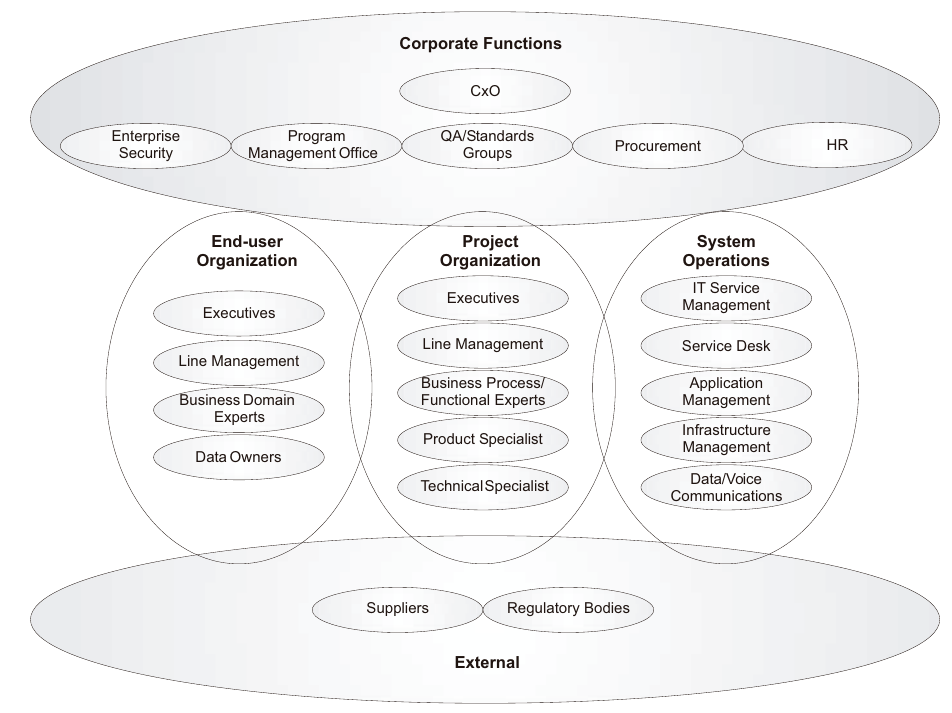
\includegraphics[width=\textwidth]{../figures/sample_stakeholders}
                    \end{center}
                \end{column}
                \begin{column}{0.5\textwidth}
                    \begin{center}
                        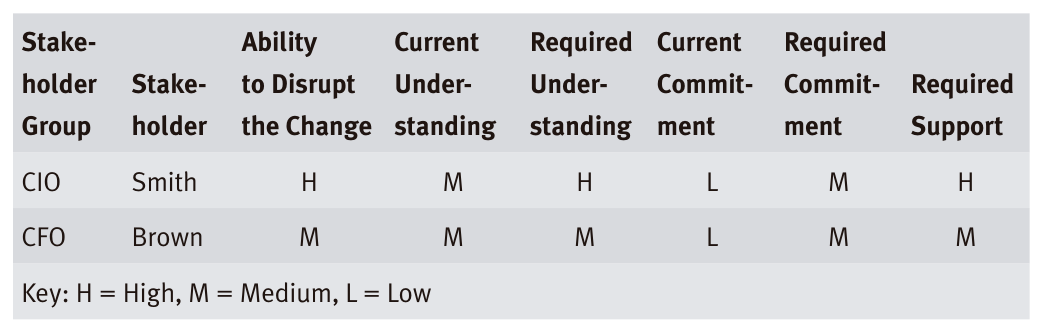
\includegraphics[width=\textwidth]{../figures/stakeholder_analysis}
                    \end{center}
                    \begin{center}
                        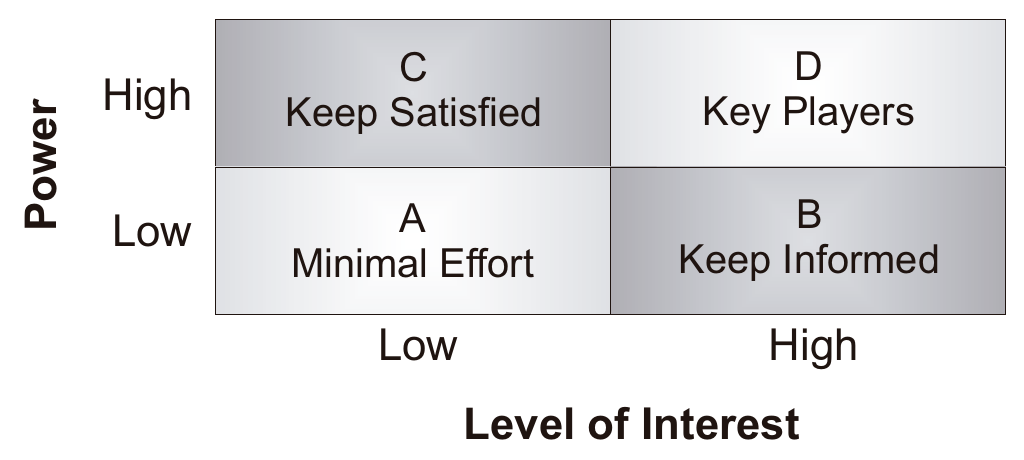
\includegraphics[width=\textwidth]{../figures/power_vs_interest}
                    \end{center}
                \end{column}
            \end{columns}

        \end{frame}
    }

    {
        \setbeamertemplate{navigation symbols}{}
        \setbeamertemplate{footline}{}
        \begin{frame}
            \frametitle{Stakeholder Map}
%            \framesubtitle{\hspace{1cm}}
            \begin{columns}
                \begin{column}{0.5\textwidth}
                    \begin{center}
                        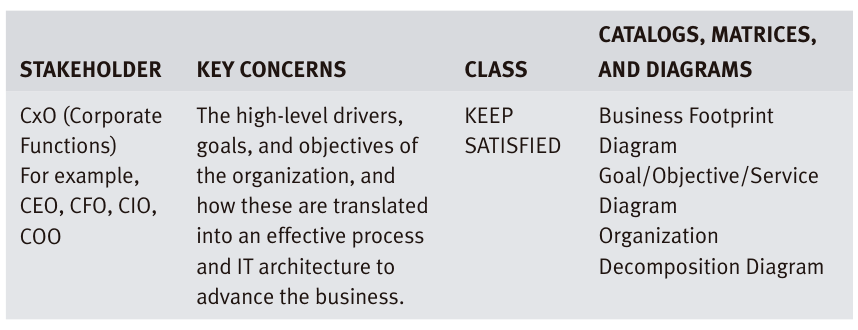
\includegraphics[width=\textwidth]{../figures/stakeholder_map_1}
                        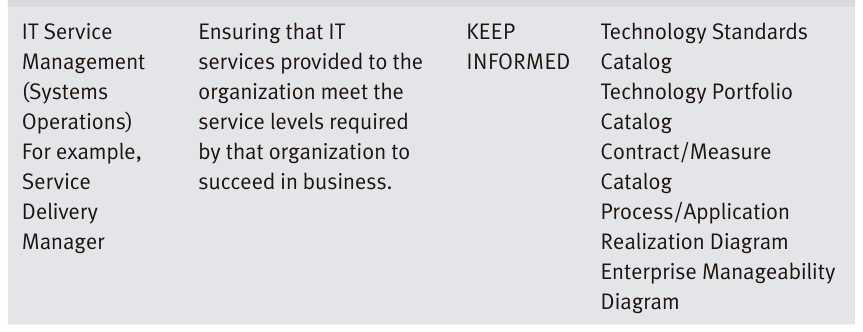
\includegraphics[width=\textwidth]{../figures/stakeholder_map_3}
                    \end{center}

                \end{column}
                \begin{column}{0.5\textwidth}
                    \begin{center}
                        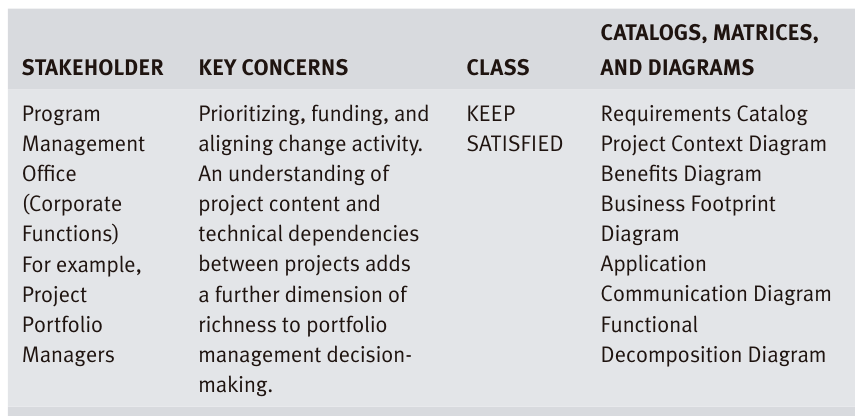
\includegraphics[width=\textwidth]{../figures/stakeholder_map_2}
                    \end{center}
                \end{column}
            \end{columns}

        \end{frame}
    }

    \begin{frame}
        \frametitle{Assessing Readiness for Transformation}

        \framesubtitle{\hspace{1cm}}
        \begin{columns}
            \begin{column}{0.5\textwidth}
                \begin{enumerate}
                    \item Vision
                    \item The desire or willingness to achieve results
                    \item Requirements
                    \item There are indications/cases in business
                    \item Funds
                    \item Sponsorship and leadership
                    \item Governance

                \end{enumerate}
            \end{column}
            \begin{column}{0.5\textwidth}
                \begin{enumerate}
                    \setcounter{enumi}{7}
                    \item Accountability (ability to be held accountable)
                    \item Workable execution approaches and models
                    \item IT capacity to execute
                    \item Company capacity to execute
                    \item The company's ability to implement and operate post-execution
                \end{enumerate}
            \end{column}
        \end{columns}
    \end{frame}

    \begin{frame}
        \frametitle{Architectural Vision}
%        \framesubtitle{\hspace{1cm}}
        \begin{enumerate}
            \item A description of the problem, including stakeholders and their concerns, as well as a list of issues/scenarios that need to be addressed.
            \item Purpose of Architectural Work Statement.
            \item Summary of views required for high-level Architecture and Business Architecture, Applications, Data, and Technology Job Requests.
            \item Business scenarios.
            \item Stakeholder needs that have been mapped and detailed.
        \end{enumerate}
    \end{frame}



    \begin{frame}
        \frametitle{Business Scenario}
%        \framesubtitle{\hspace{1cm}}
        \begin{enumerate}
            \item \textbf{Problem}.
            Identify, document, and rank the issues driving the project.
            \item \textbf{Business and Technical Environment}.
            Document as a high-level architectural model the business and technical environments in which the problem situation occurs.
            \item \textbf{Goals and Measures of Success}.
            Identify and document the desired goals, outcomes of successfully addressing the problem.
            \item \textbf{Human Actor}.
            Identify human actors and their place in the business model, human participants and their roles.

        \end{enumerate}
    \end{frame}

    \begin{frame}
        \frametitle{Business Scenario}
%        \framesubtitle{\hspace{1cm}}
        \begin{enumerate}
            \setcounter{enumi}{4}
            \item \textbf{Computer Actor}.
            Identify computer actors and their place in the technology model, computing elements, and their roles.
            \item \textbf{Roles and Responsibilities}.
            Identify and document the roles, responsibilities, and measures of success per actor, required scripts per actor, and the desired outcome of properly handling the situation.
            \item \textbf{Revision}.
            Check for suitability of purpose to inspire subsequent architectural work, and refine only if necessary.
        \end{enumerate}
    \end{frame}

    \begin{frame}
        \frametitle{Architectural Statement of Work Document}
        \framesubtitle{\hspace{1cm}}
        \vspace{20pt}
        \begin{enumerate}
            \item Title
            \item Architectural Project Requests and Background
            \item Architectural Project Description and Scope
            \item Architectural Vision Overview
            \item Specific Scope Change Procedures
            \item Roles, Responsibilities, and Deliverables
            \item Acceptance Criteria and Procedures
            \item Architectural Project Plans and Schedules
            \item Approval
        \end{enumerate}
    \end{frame}

\begin{frame}{Preliminary Phase vs. Architecture Vision}
	\begin{columns}[t]
		\column{0.5\textwidth}
		\textbf{Preliminary Phase}
		\begin{itemize}
			\item Establishing the architecture framework and principles.
			\item Defining architecture governance.
			\item Setting up tools, processes, and organizational structures for architecture work.
		\end{itemize}
		
		\column{0.5\textwidth}
		\textbf{Architecture Vision}
		\begin{itemize}
			\item Developing a high-level vision of the architecture.
			\item Defining the project scope, objectives, constraints, readiness, and expectations.
			\item Conducting initial stakeholder analysis.
			\item Creating a high-level description of the baseline and target architecture.
		\end{itemize}
	\end{columns}
\end{frame}

    \begin{frame}
        \frametitle{Summary}
%        \framesubtitle{\hspace{1cm}}
        \begin{enumerate}
            \item The Architectural Vision Phase is the first step in the TOGAF Architectural Development Method, where we define the scope, identify stakeholders, and define a high-level architectural vision.
            \item This phase is critical to ensuring that the architectural project has the right support and direction from the start.
        \end{enumerate}

    \end{frame}

\end{document}